Descriptive statistics confirmed that all three canonical stylized facts were present in both the in-sample (2014--2024, $T = 2{,}766$) and out-of-sample (2025, $T = 219$) windows (Table~\ref{tab:descriptive}): excess kurtosis of 7.7 (IS) and 6.2 (OoS) with Jarque-Bera rejection ($p < 0.001$), persistent volatility clustering (Ljung-Box on $|G_t|$ rejected, $p < 0.001$), and near-zero linear autocorrelation in raw returns.
These regularities are visualized in Figure~\ref{fig:stylized_facts}.

\begin{table}[t]
\centering
\caption{Descriptive statistics and stylized-facts tests for SPY daily excess growth rates. IS: 2014--2024 ($T = 2{,}766$); OoS: 2025 ($T = 219$). JB = Jarque-Bera normality test. LB = Ljung-Box autocorrelation test at lag~20. $^*$ denotes rejection at $\alpha = 0.05$.}
\label{tab:descriptive}
\begin{tabular}{lcc}
\toprule
Statistic & IS Observed & OoS Observed \\
\midrule
Mean (annualized) & 0.11 & 0.13 \\
Std Dev (annualized) & 2.14 & 2.31 \\
Skewness & $-0.753$ & $-1.071$ \\
Excess Kurtosis & 7.707 & 6.242 \\
JB normality test & reject$^*$ ($p < 0.001$) & reject$^*$ ($p < 0.001$) \\
LB test on $G_t$ (lag 20) & reject$^*$ (145.3) & fail to reject (28.1) \\
LB test on $|G_t|$ (lag 20) & reject$^*$ (3057.9) & reject$^*$ (150.4) \\
\bottomrule
\end{tabular}
\end{table}

\begin{figure}[t]
\centering

\includegraphics[width=\textwidth]{sections/figs/Fig-1-Stylized-Facts.pdf}
\caption{Empirical stylized facts of SPY daily excess growth rates (2014--2024). Panel~(a) shows the leptokurtic marginal distribution; the Laplace fit substantially outperforms the Gaussian. Panel~(b) confirms heavy tails via a normal Q-Q plot. Panel~(c) shows near-zero autocorrelation of raw returns. Panel~(d) shows the persistent autocorrelation of absolute returns that characterizes volatility clustering.}
\label{fig:stylized_facts}
\end{figure}

\subsection{Baum-Welch Training and Model Internals}

We trained continuous Gaussian HMMs for $K \in \{3, 6, 9, 11, 13\}$ states using the Baum-Welch algorithm with \texttt{max\_iter}~=~60.
All models converged within the iteration budget, with log-likelihood plateauing after 20--40 iterations (Figure~S\ref{fig:convergence}, Supplemental).

Figure~\ref{fig:model_internals} shows the fitted model internals for $K = 13$: the learned emission distributions span the full range of observed returns, with tail states capturing extreme crash and boom regimes.
The transition matrix exhibits a dominant near-diagonal band reflecting short-range regime persistence.
Critically, the natural residence time $1/(1 - T_{kk})$ for all states---including the tails---is only 1--2 steps under pure Markov dynamics, motivating the jump-duration extension.

\begin{figure}[t]
\centering
\begin{subfigure}[b]{0.48\textwidth}
    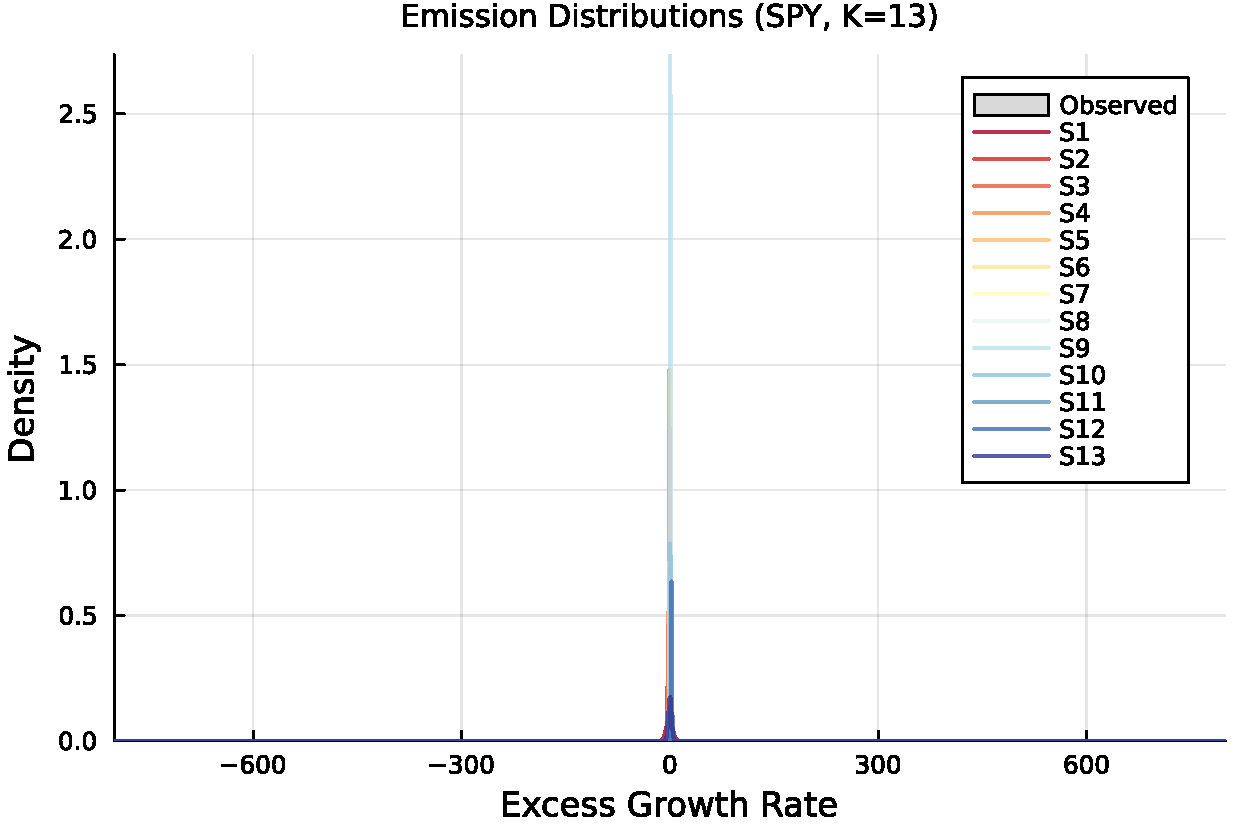
\includegraphics[width=\textwidth]{sections/figs/Fig-Emission-PDFs-K13.pdf}
    \caption{Emission distributions ($K = 13$)}
\end{subfigure}
\hfill
\begin{subfigure}[b]{0.48\textwidth}
    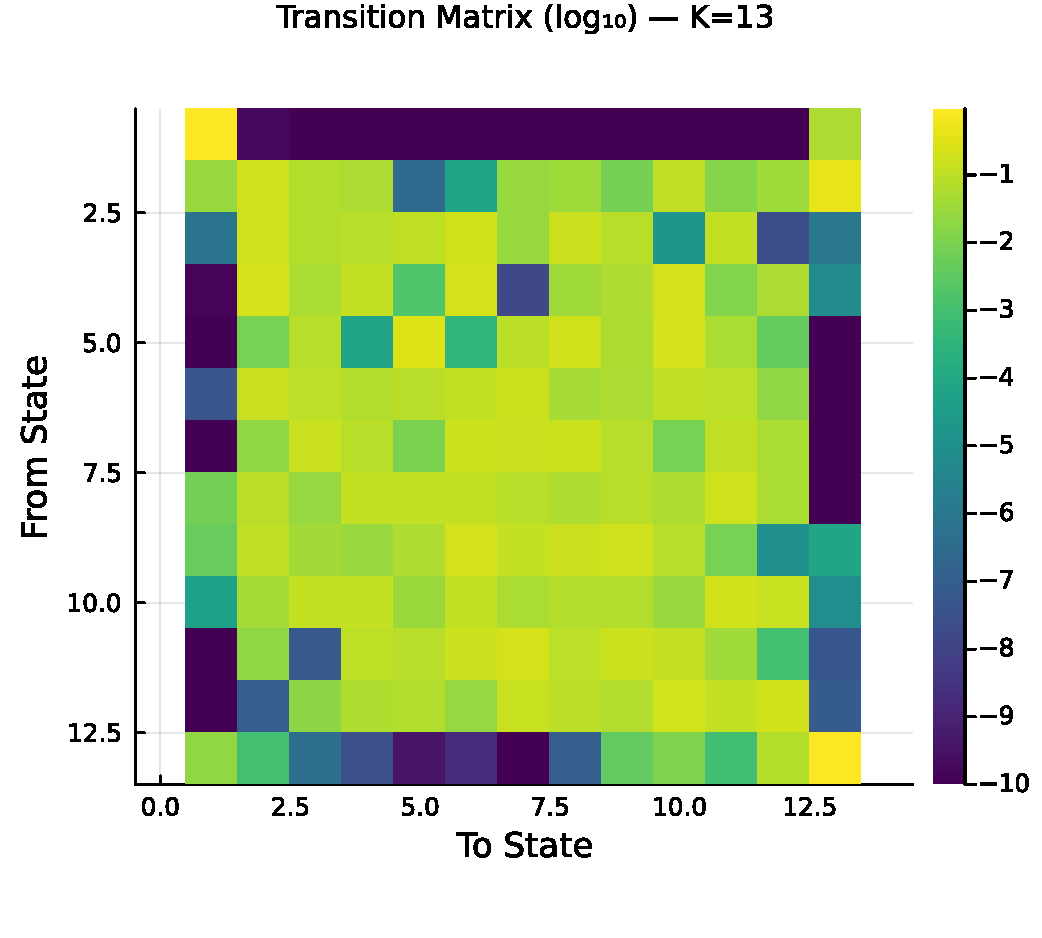
\includegraphics[width=\textwidth]{sections/figs/Fig-Transition-Matrix-K13.pdf}
    \caption{Transition matrix (log$_{10}$ scale)}
\end{subfigure}
\caption{Fitted model internals for SPY with $K = 13$ states. (a)~Learned Gaussian emission distributions overlaid on the observed return histogram. (b)~Empirical transition matrix in log$_{10}$ color scale; the dominant near-diagonal band reflects short-range regime persistence.}
\label{fig:model_internals}
\end{figure}

\subsection{Jump Hyperparameter Optimization}

For each state resolution $K$, a grid search over $\epsilon$ and $\lambda$ identified the optimal jump parameters (Table~\ref{tab:sensitivity}).
The optimal $\epsilon^* = 10^{-4}$ was consistently selected for $K \in \{3, 9, 11, 13\}$, with $K = 6$ preferring $\epsilon^* = 10^{-3}$.
The optimal $\lambda^*$ varied across state resolutions, ranging from 10 ($K = 3, 11$) to 130 ($K = 6$), indicating that the mean jump duration adapts to the granularity of the state space.

\subsection{In-Sample Model Comparison}

Table~\ref{tab:model_comparison} and Figure~\ref{fig:is_comparison} present the in-sample validation results for $K = 13$.
Bootstrap resampling set the non-parametric ceiling (99.8\% KS), while Gaussian i.i.d.\ sampling confirmed that thin-tailed models are categorically inadequate (0\% KS).
Laplace i.i.d.\ achieved 98.2\% KS but produced near-zero kurtosis excess relative to the observed 7.7, indicating that while the marginal shape matched, the model lacked the dynamic structure to reproduce temporal patterns.

Both CHMM variants achieved KS pass rates above 91\%, with CHMM-NJ at 94.6\% and CHMM-WJ at 91.5\%.
The slight decrease for CHMM-WJ reflects the jump mechanism occasionally overweighting tail states, a cost of improved temporal fidelity.
The Wasserstein-1 and Hellinger distances for both CHMM variants were comparable to the bootstrap baseline, confirming high distributional fidelity.

The kurtosis gap between simulated (4.2) and observed (7.7) indicates that Gaussian emissions underestimate tail weight relative to the Student-$t$ emissions used in the discrete model \citep{alswaidan2026hybrid}.
This motivates future work on heavy-tailed emission distributions within the Baum-Welch framework.

\begin{table}[t]
\centering
\caption{In-sample and out-of-sample model comparison for SPY at $K = 13$ (1{,}000 simulated paths, $\alpha = 0.05$). Bootstrap: i.i.d.\ resample of training data. Gaussian/Laplace: i.i.d.\ draws from MLE-fitted distributions. CHMM-NJ: continuous HMM without jumps. CHMM-WJ: continuous HMM with Poisson jump-duration extension ($\epsilon^* = 10^{-4}$, $\lambda^* = 100$).}
\label{tab:model_comparison}
\small
\begin{tabular}{lcccccc}
\toprule
& \multicolumn{3}{c}{In-Sample (2{,}766 days)} & \multicolumn{3}{c}{Out-of-Sample (219 days)} \\
\cmidrule(lr){2-4} \cmidrule(lr){5-7}
Model & KS (\%) $\uparrow$ & Kurtosis $\approx$ & $W_1$ $\downarrow$ & KS (\%) $\uparrow$ & Kurtosis $\approx$ & $W_1$ $\downarrow$ \\
\midrule
\textit{Observed} & --- & 7.71 & --- & --- & 6.24 & --- \\
Bootstrap & 99.8 & 7.52 & 0.061 & 99.3 & 5.52 & --- \\
Gaussian & 0.0 & $-0.01$ & 0.400 & 74.4 & $-0.04$ & --- \\
Laplace & 98.2 & 2.96 & 0.120 & 97.5 & 2.67 & --- \\
CHMM-NJ & 94.6 & 4.22 & 0.109 & 94.1 & 3.01 & 0.371 \\
CHMM-WJ & 91.5 & 4.17 & 0.112 & 93.6 & 2.84 & 0.385 \\
\bottomrule
\end{tabular}
\end{table}

\begin{figure}[t]
\centering
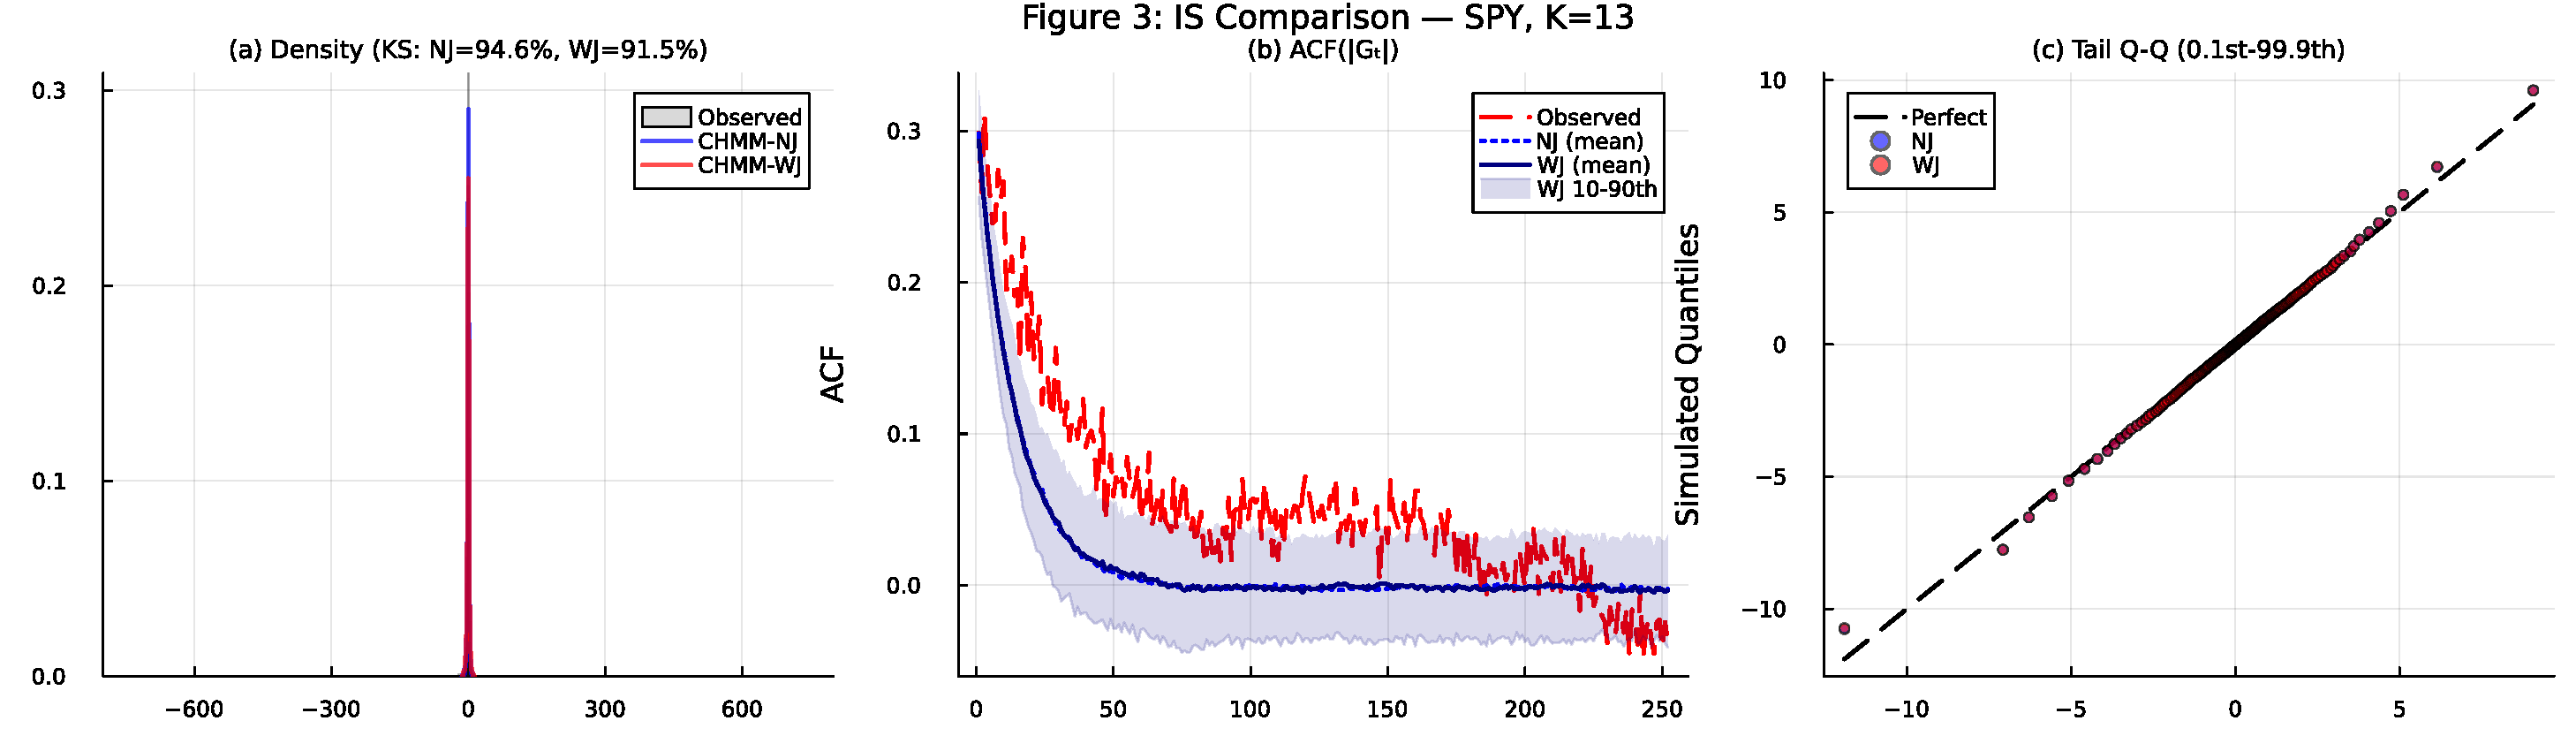
\includegraphics[width=\textwidth]{sections/figs/Fig-3-IS-Comparison-K13.pdf}
\caption{In-sample model comparison for SPY ($K = 13$, 1{,}000 paths). (a)~Marginal density with KS pass rates annotated. (b)~ACF of absolute excess growth rates; CHMM-NJ shows near-zero ACF (no volatility clustering), while CHMM-WJ partially reproduces the observed slow decay. (c)~Tail Q-Q plot comparing simulated quantiles to observed.}
\label{fig:is_comparison}
\end{figure}

\subsection{Out-of-Sample Evaluation}

The out-of-sample results (Table~\ref{tab:model_comparison}, Figure~\ref{fig:oos_validation}) demonstrated robust generalization.
CHMM-NJ achieved 94.1\% KS and CHMM-WJ achieved 93.6\% KS on the held-out 2025 data, comparable to the in-sample performance.
This contrasts with the discrete model's finding that IS-calibrated jump parameters showed mild overfitting \citep{alswaidan2026hybrid}; the continuous model's Baum-Welch training may produce more generalizable emission parameters.

\begin{figure}[t]
\centering
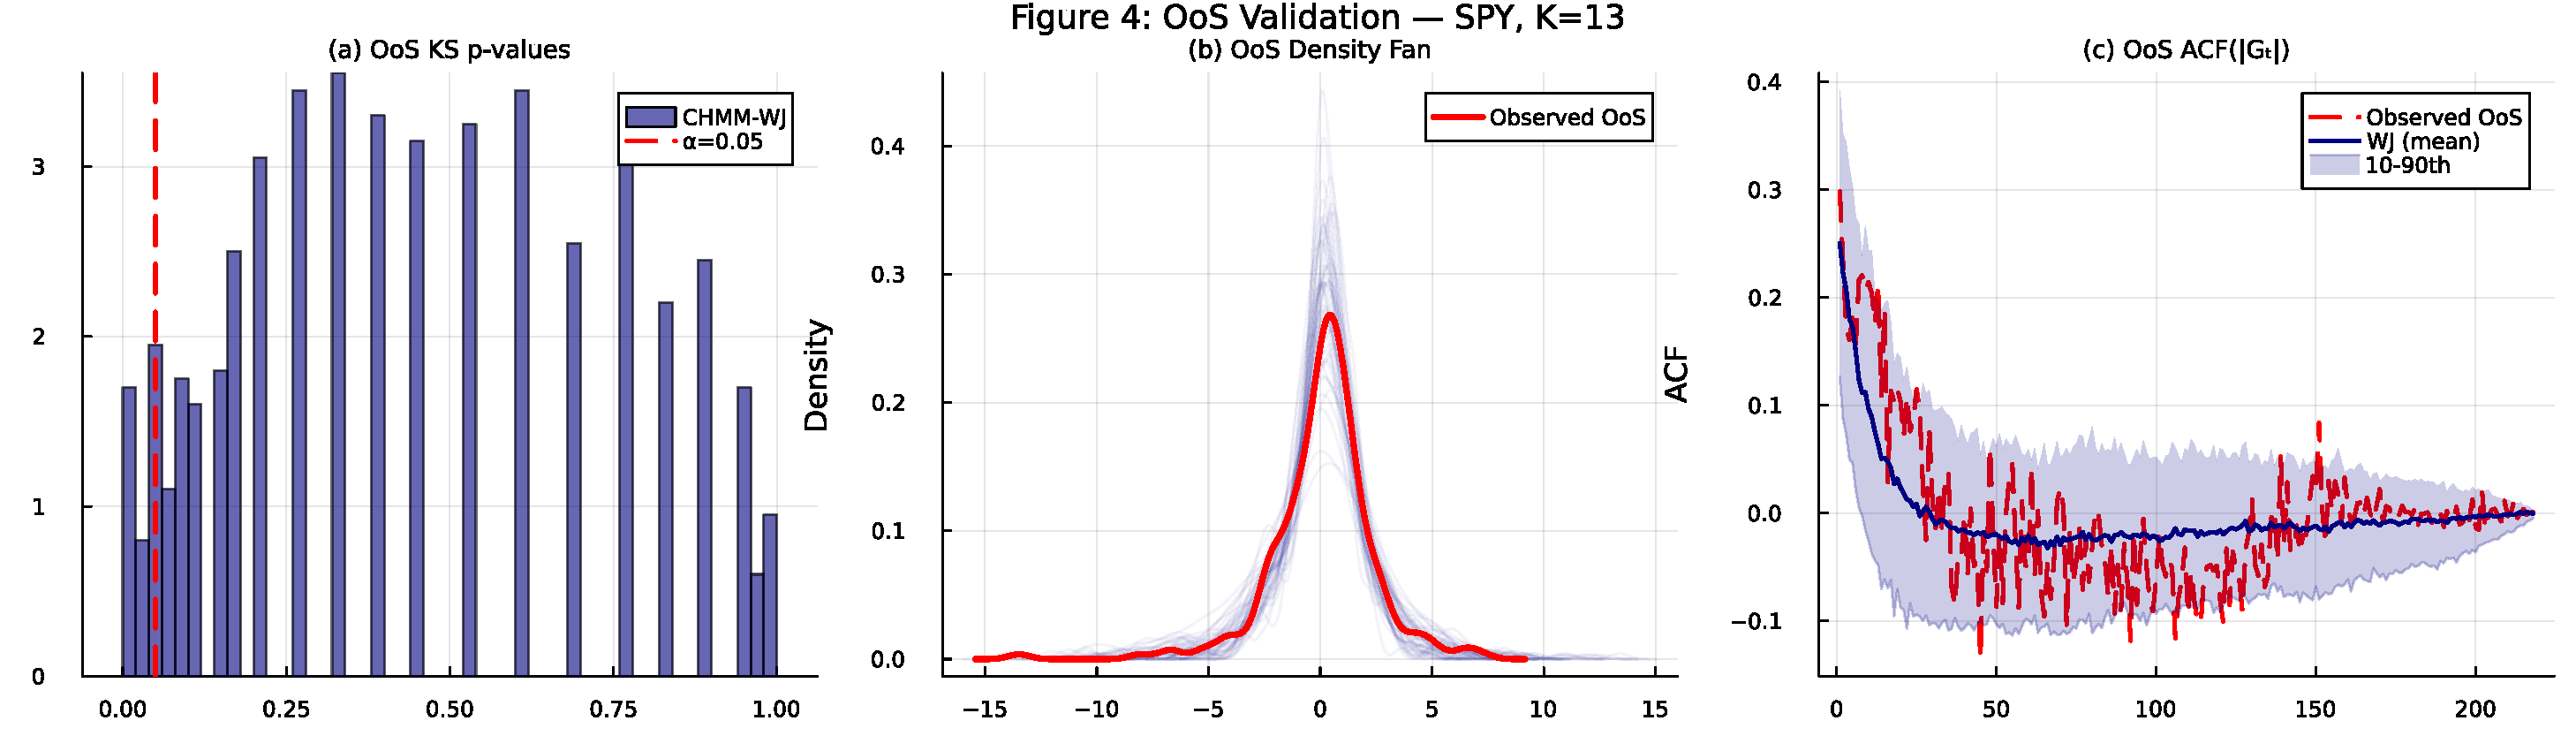
\includegraphics[width=\textwidth]{sections/figs/Fig-4-OoS-Validation-K13.pdf}
\caption{Out-of-sample validation of CHMM-WJ ($K = 13$, $\alpha = 0.05$). (a)~KS $p$-values for 1{,}000 OoS paths. (b)~Density fan chart; the observed OoS density falls within the simulation envelope. (c)~OoS ACF of $|G_t|$ with 10th--90th percentile band.}
\label{fig:oos_validation}
\end{figure}

\subsection{State Resolution Sensitivity}

Table~\ref{tab:sensitivity} reports the sensitivity of model performance to the number of hidden states $K$.
KS pass rates improved monotonically from 87.1\% ($K = 3$) to 94.6\% ($K = 13$) for CHMM-NJ, confirming that finer state resolution produces better distributional fidelity.
ACF-MAE remained stable across all $K$ values (0.045--0.050), indicating that the jump mechanism's effectiveness is largely independent of state count.
Wasserstein-1 and Hellinger distances showed similar stability, with modest improvements at higher $K$.

\begin{table}[t]
\centering
\caption{State resolution sensitivity for SPY (1{,}000 paths, $\alpha = 0.05$). $\epsilon^*$ and $\lambda^*$ are the grid-search optimal jump parameters for each $K$.}
\label{tab:sensitivity}
\small
\begin{tabular}{cccrrrrrrrr}
\toprule
& & & \multicolumn{2}{c}{KS IS (\%)} & \multicolumn{2}{c}{KS OoS (\%)} & \multicolumn{2}{c}{ACF-MAE} & \multicolumn{2}{c}{$W_1$} \\
\cmidrule(lr){4-5} \cmidrule(lr){6-7} \cmidrule(lr){8-9} \cmidrule(lr){10-11}
$K$ & $\epsilon^*$ & $\lambda^*$ & NJ & WJ & NJ & WJ & NJ & WJ & NJ & WJ \\
\midrule
3  & $10^{-4}$ & 10  & 87.1 & 89.1 & 89.5 & 93.7 & 0.045 & 0.046 & 0.121 & 0.120 \\
6  & $10^{-3}$ & 130 & 92.0 & 91.6 & 92.8 & 94.6 & 0.049 & 0.050 & 0.105 & 0.108 \\
9  & $10^{-4}$ & 55  & 92.9 & 91.7 & 93.5 & 92.1 & 0.047 & 0.047 & 0.112 & 0.115 \\
11 & $10^{-4}$ & 10  & 93.5 & 95.0 & 92.6 & 92.5 & 0.049 & 0.050 & 0.113 & 0.110 \\
13 & $10^{-4}$ & 100 & 94.6 & 91.5 & 94.1 & 93.6 & 0.048 & 0.048 & 0.109 & 0.112 \\
\bottomrule
\end{tabular}
\end{table}

\subsection{Cross-Asset Generalization}

To assess whether the framework generalized beyond SPY, we fitted independent CHMM models to three equities spanning distinct risk profiles: NVDA (high-beta technology), JNJ (low-beta health care), and JPM (moderate-beta financials).
Table~\ref{tab:cross_asset} reports the results.

CHMM-NJ achieved KS pass rates above 98\% for all three tickers in-sample, confirming that the Baum-Welch training captured the marginal distribution of individual equities with diverse tail characteristics.
Out-of-sample, NVDA maintained strong fidelity (98.5\% KS), while JNJ and JPM showed more degradation (70--78\% KS), reflecting asset-specific regime shifts in 2025 that the stationary IS-calibrated parameters could not fully capture.
The CHMM-WJ results showed that the jump mechanism's effectiveness varied by asset: NVDA and JPM showed KS degradation from jumps (consistent with the SPY finding), while the ACF-MAE consistently improved, confirming the distributional-temporal tradeoff.

\begin{table}[t]
\centering
\caption{Cross-asset generalization ($K = 13$, 1{,}000 paths, $\alpha = 0.05$). Each ticker was fitted independently.}
\label{tab:cross_asset}
\small
\begin{tabular}{llrrrrrr}
\toprule
& & \multicolumn{2}{c}{KS (\%)} & & & \\
\cmidrule(lr){3-4}
Ticker & Model & IS & OoS & Kurt (obs) & Kurt (sim) & ACF-MAE & $W_1$ IS \\
\midrule
\multirow{2}{*}{NVDA} & CHMM-NJ & 98.0 & 98.5 & \multirow{2}{*}{5.0} & 3.32 & 0.042 & 0.236 \\
                      & CHMM-WJ & 61.2 & 92.4 &                       & 3.21 & 0.039 & 0.381 \\
\midrule
\multirow{2}{*}{JNJ}  & CHMM-NJ & 99.4 & 70.0 & \multirow{2}{*}{8.6} & 5.30 & 0.031 & 0.091 \\
                      & CHMM-WJ & 0.0  & 72.3 &                       & 3.92 & 0.028 & 0.487 \\
\midrule
\multirow{2}{*}{JPM}  & CHMM-NJ & 98.7 & 77.8 & \multirow{2}{*}{8.0} & 4.41 & 0.044 & 0.168 \\
                      & CHMM-WJ & 64.9 & 70.0 &                       & 4.09 & 0.042 & 0.225 \\
\bottomrule
\end{tabular}
\end{table}
